% file: PGL_4_2_sims_1.tex
% created by Orbiter tikz interface
% creation date: Thu Dec 17 16:59:38 MST 2020
% DeviceCoordinates 0 0 1000000 1000000
% UserCoordinates 0 0 10000 10000
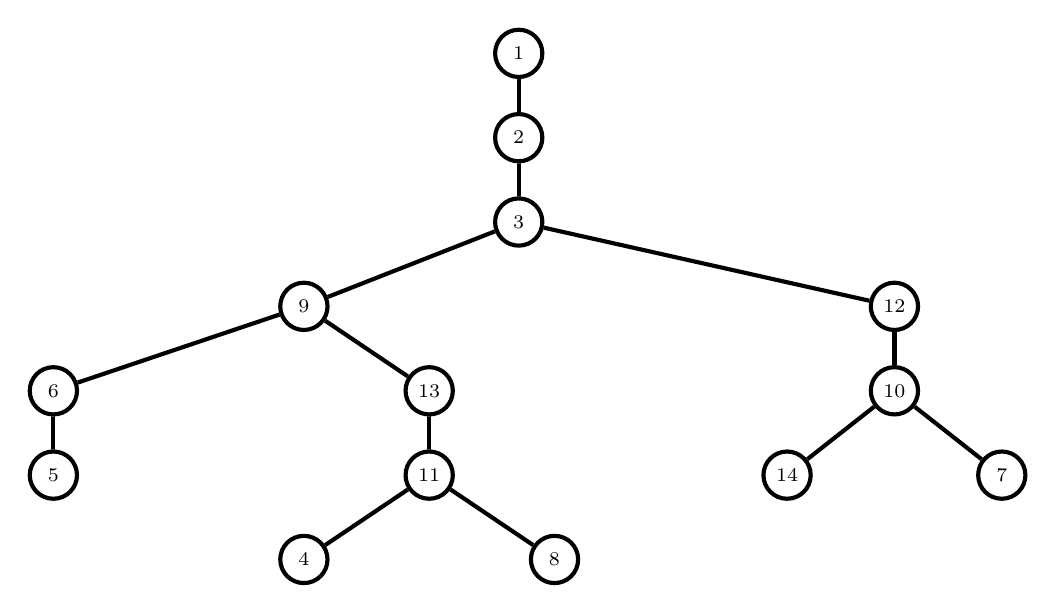
\begin{tikzpicture}[scale=0.45,line width = 1.5pt]
\draw [] (16.6667,32.14) -- (16.6667,29.76);
\draw [] (16.6667,29.76) -- (16.6667,27.38);
\draw [] (16.6667,27.38) -- (10.6033,25);
\draw [] (16.6667,27.38) -- (27.27,25);
\draw [] (10.6033,25) -- (3.53333,22.6167);
\draw [] (10.6033,25) -- (14.14,22.6167);
\draw [] (27.27,25) -- (27.27,22.6167);
\draw [] (3.53333,22.6167) -- (3.53333,20.2367);
\draw [] (14.14,22.6167) -- (14.14,20.2367);
\draw [] (27.27,22.6167) -- (24.24,20.2367);
\draw [] (27.27,22.6167) -- (30.3,20.2367);
\draw [] (14.14,20.2367) -- (10.6033,17.8567);
\draw [] (14.14,20.2367) -- (17.6767,17.8567);
\filldraw[color=white] (16.6667,32.14) circle [radius = 0.666667cm];
\draw (16.6667,32.14) circle [radius = 0.666667cm];
\draw (16.6667,32.14) node{{\scriptsize 1}};
\filldraw[color=white] (16.6667,29.76) circle [radius = 0.666667cm];
\draw (16.6667,29.76) circle [radius = 0.666667cm];
\draw (16.6667,29.76) node{{\scriptsize 2}};
\filldraw[color=white] (16.6667,27.38) circle [radius = 0.666667cm];
\draw (16.6667,27.38) circle [radius = 0.666667cm];
\draw (16.6667,27.38) node{{\scriptsize 3}};
\filldraw[color=white] (10.6033,25) circle [radius = 0.666667cm];
\draw (10.6033,25) circle [radius = 0.666667cm];
\draw (10.6033,25) node{{\scriptsize 9}};
\filldraw[color=white] (27.27,25) circle [radius = 0.666667cm];
\draw (27.27,25) circle [radius = 0.666667cm];
\draw (27.27,25) node{{\scriptsize 12}};
\filldraw[color=white] (3.53333,22.6167) circle [radius = 0.666667cm];
\draw (3.53333,22.6167) circle [radius = 0.666667cm];
\draw (3.53333,22.6167) node{{\scriptsize 6}};
\filldraw[color=white] (14.14,22.6167) circle [radius = 0.666667cm];
\draw (14.14,22.6167) circle [radius = 0.666667cm];
\draw (14.14,22.6167) node{{\scriptsize 13}};
\filldraw[color=white] (27.27,22.6167) circle [radius = 0.666667cm];
\draw (27.27,22.6167) circle [radius = 0.666667cm];
\draw (27.27,22.6167) node{{\scriptsize 10}};
\filldraw[color=white] (3.53333,20.2367) circle [radius = 0.666667cm];
\draw (3.53333,20.2367) circle [radius = 0.666667cm];
\draw (3.53333,20.2367) node{{\scriptsize 5}};
\filldraw[color=white] (14.14,20.2367) circle [radius = 0.666667cm];
\draw (14.14,20.2367) circle [radius = 0.666667cm];
\draw (14.14,20.2367) node{{\scriptsize 11}};
\filldraw[color=white] (24.24,20.2367) circle [radius = 0.666667cm];
\draw (24.24,20.2367) circle [radius = 0.666667cm];
\draw (24.24,20.2367) node{{\scriptsize 14}};
\filldraw[color=white] (30.3,20.2367) circle [radius = 0.666667cm];
\draw (30.3,20.2367) circle [radius = 0.666667cm];
\draw (30.3,20.2367) node{{\scriptsize 7}};
\filldraw[color=white] (10.6033,17.8567) circle [radius = 0.666667cm];
\draw (10.6033,17.8567) circle [radius = 0.666667cm];
\draw (10.6033,17.8567) node{{\scriptsize 4}};
\filldraw[color=white] (17.6767,17.8567) circle [radius = 0.666667cm];
\draw (17.6767,17.8567) circle [radius = 0.666667cm];
\draw (17.6767,17.8567) node{{\scriptsize 8}};
\end{tikzpicture}
